\documentclass{article}

    % Input language encoding
    %\usepackage[utf8]{inputenc}
   
    % Output languages
    %\usepackage[greek, english]{babel}
    % \usepackage{alphabeta}
    
    % Fonts
    %\usepackage[T1,LGR]{fontenc}
    \usepackage{lmodern}

    % Images
    \usepackage{graphicx}
    \usepackage{float}
    \usepackage{caption}
    \usepackage{subcaption}

    % Math
    \usepackage{amsmath}

    % Paragraph Formatting
    \usepackage{parskip}

    % Code
    \usepackage{listings}

        

    \DeclareMathSizes{10}{10}{10}{10}
    \setlength{\parindent}{0cm}

    \title{Excercise 1.2-2}

\begin{document}

\pagenumbering{gobble}
\date{}
\author{}

\maketitle

In this case, we need to figure out when $ 8 * n^{2} \leq 64* n * \lg{n} $.

By plotting it in Matlab, we have the Figure \ref{fig:plot1}:

\begin{figure}
    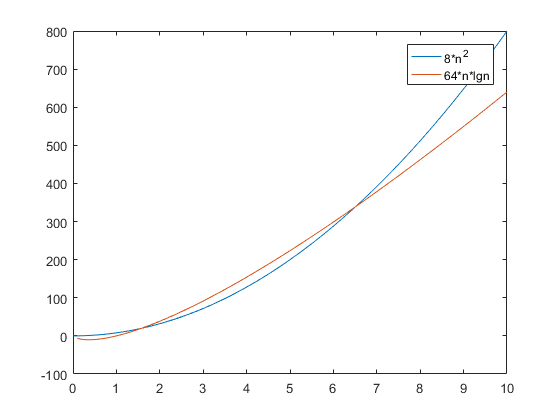
\includegraphics[width=10cm]{images/1-2-2.png}
    \centering
    \caption{Our plot}
    \label{fig:plot1}
\end{figure}

The Matlab code we used is the following:

\begin{lstlisting}[language=Matlab]
    x = linspace(0,10);
    y1 = 8 * x.^2;
    y2 = 64 * x .* log10(x);
    figure();
    plot(x,y1,x,y2);
    legend('8*n^2','64*n*lgn');
\end{lstlisting}

As we see the period that $8*n^{2}$ is faster than $64*n*\lg{n}$ is between 1 and 6. This is easy to calculate from seing the plot and a little bit of trial and error in the edges. \textbf{Keep in mind, that since we are talking about inputs, we are only interested in intergers.}
\end{document}